\documentclass{article}
\usepackage[utf8]{inputenc}
\usepackage[T1]{fontenc}
\usepackage{geometry}
\usepackage{enumitem}
\usepackage{graphicx}

\geometry{margin=0.75in}

\begin{document}

\title{\textbf{Specyfikacja funkcjonalna}
\\ \large{\textit{Ganics}}}
\author{\textbf{Adrian Chmiel}}
\date{4 czerwca 2024}
\maketitle

\section{Cel projektu}
Celem projektu jest wykorzystanie sieci GAN do generacji obrazów ze zmienionym stylem. Program oferuje dwa możliwe style konwersji:
\begin{enumerate}[label=\arabic*.]
    \setlength\itemsep{0pt}
    \item \textbf{Vincent Van Gogh Art} - obrazy będą przypominać dzieła sztuki Vincenta Van Gogha
    \item \textbf{Cartoon} - obrazy będą przypominać zdjęcia pochodzące z kreskówki, bądź komiksu
\end{enumerate}

\section{Informacje ogólne}
Program został napisany w języku Python w wersji 3.10. Program korzysta z następujących bibliotek:
\begin{itemize}
    \setlength\itemsep{0pt}
    \item \textbf{matplotlib} - do tworzenia wykresów oraz wizualizacji danych
    \item \textbf{numpy} - do wykonywania operacji na macierzach
    \item \textbf{opencv-python} - do przetwarzania obrazów
    \item \textbf{pandas} - do analizy danych
    \item \textbf{pillow} - do przetwarzania obrazów
    \item \textbf{pydot} - do wizualizacji struktury modeli
    \item \textbf{tensorflow} - do tworzenia oraz trenowania modeli sieci GAN
    \item \textbf{tkinter} - do stworzenia prostego interfejsu graficznego
    \item \textbf{tqdm} - do wyświetlania postępu w uczeniu modelu
\end{itemize}

\section{Uruchamianie programu}
Aby uruchomić aplikację bezpośrednio z \textbf{kodu źródłowego}, zalecanym podejściem jest utworzenie nowego wirtualnego środowiska oraz zainstalowanie w nim wymaganych bibliotek/pakietów.
Zakładając, że korzystamy z \textit{conda} możemy to wykonać następującymi komendami:
\begin{verbatim}
conda create -n Ganics python=3.10 -y
conda activate Ganics
conda install jupyter
pip install -r requirements.txt
\end{verbatim}
Instalację jupytera można pominąć, jeśli nie zamierzamy korzystać z notebooków.
\vspace{3mm} \\
Dla posiadaczy kart graficznych NVIDIA warto również wykonać następującą komendę, która umożliwi korzystanie z CUDA:
\begin{verbatim}
conda install -c conda-forge cudatoolkit=11.2 cudnn=8.1.0 -y
\end{verbatim}
Program można uruchomić poprzez wywołanie pliku \textbf{\textit{main.py}}:
\begin{verbatim}
python src/main.py
\end{verbatim}

\section{Interfejs graficzny}
Interfejs graficzny programu został stworzony przy użyciu biblioteki \textit{tkinter}. Umożliwia on:
\begin{itemize}
    \setlength\itemsep{0pt}
    \item Wybór pliku wejściowego
    \item Wybór stylu konwersji
    \item Konwersję oraz zapisanie obrazu
    \item Podgląd obrazu przed oraz po konwersji
\end{itemize}
Przykładowy zrzut ekranu interfejsu graficznego znajduje się poniżej:
\vspace{3mm} \\
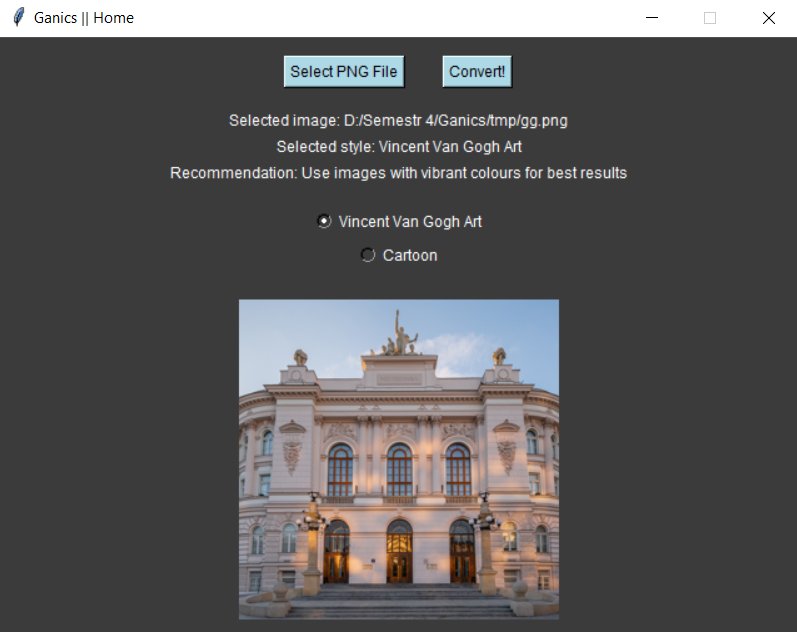
\includegraphics[width=0.5\textwidth]{../imgs/gui.png}

\section{Pliki wejściowe oraz wyjściowe}
\begin{enumerate}[label=\arabic*.]
    \item \textbf{Główna aplikacja} \\
Program umożliwia wybranie ścieżki do pliku wejściowego, który będzie poddany konwersji. Warto zaznaczyć, że plik wejściowy musi być obrazem w formacie \textit{.jpg}, \textit{.jpeg} lub \textit{.png}.
\vspace{3mm} \\
Natomiast plikiem wyjściowym niezależnie od początkowego formatu jest zawsze obraz w formacie \textit{.png} o rozdzielczości \textit{512x512}.
    \item \textbf{Notebooki} \\
W przypadku notebooków jako wejście podajemy całe zbiory obrazów (więcej informacji poniżej), które zostaną wykorzystane do nauki modelu. Jako wyjście otrzymujemy wizualizacje obrazujące, jak model sprawuje się po zakończeniu nauki oraz wyeksportowany plik z wagami modelu, który później jest wykorzystywany jako komponent głównej aplikacji.
\end{enumerate}

\section{Sposób działania aplikacji}
Zamysł działania aplikacji widoczny jest poniżej:
\begin{enumerate}[label=\arabic*.]
    \item Wybór pliku oraz stylu konwersji
    \item Translacja stylu obrazu przy wykorzystaniu \textbf{CycleGAN} \\
\textit{Obraz powstały w tym procesie ma rozdzielczość 256x256.}
    \item Upscaling obrazu przy wykorzystaniu \textbf{SRGAN} do rozdzielczości 512x512
    \item Zapisanie obrazu w formacie \textit{.png}
\end{enumerate}
Istotnym faktem jest, że aplikacja \textbf{nie zadziała}, jeżeli nie znajdzie odpowiednich wag modelu, o czym użytkownik zostanie poinformowany błędem.
W takim wypadku należy uruchomić notebooki, aby nauczyć model, bądź pobrać gotowe pliki dostępne na \textit{Google Drive} pod linkiem znajdującym się w pliku \textit{how\_to\_get\_models.md}. 

\section{Teoria}
Program opiera się na dwóch modelach sieci GAN:
\begin{itemize}
    \setlength\itemsep{0pt}
    \item \textbf{CycleGAN}
    \item \textbf{SRGAN} (z dyskryminatorem \textit{PatchGAN})
\end{itemize}
\textbf{GAN} \textit{(Generative Adversarial Network)} to rodzaj sztucznej sieci neuronowej, która składa się z dwóch modeli: \textbf{generatora} oraz \textbf{dyskryminatora}.
Generator ma za zadanie generować nowe obrazy, które są podobne do tych ze zbioru danych, natomiast dyskryminator ma za zadanie rozróżniać, czy obraz pochodzi z generatora, czy ze zbioru danych.
Proces szkolenia polega na rywalizacji obu modeli, gdzie generator stara się oszukać dyskryminator, a dyskryminator stara się nauczyć rozróżniać obrazy.
W efekcie końcowym generator jest w stanie generować obrazy bardzo podobne do tych ze zbioru danych.
\vspace{3mm} \\
Więcej informacji na temat działania tych modeli dostępne jest w dokumencie: \textit{Notatka\_o\_GANach.pdf}

\section{Zbiory danych}
Aby uzyskać zbiory danych do nauki modeli można wypakować dostępne pliki \textit{.zip}, które zawierają wyselekcjonowane przeze mnie obrazy z wymienionych poniżej zbiorów danych. Alternatywną opcją jest skorzystanie z linków do tych zbiorów znajdujących się w pliku \textit{README.md}. To podejście umożliwi samodzielny wybór zdjęć, które posłużą do trenowania.
\vspace{3mm} \\
Zbiory danych, które zostały wykorzystane do nauki modeli to:
\begin{itemize}
    \item \textbf{Familyguy} (ze zbioru Cartoon Classification) \\
Wykorzystany do szkolenia CycleGAN odpowiedzialnego za konwersję stylu na kreskówkę, bądź komiks.
    \item \textbf{VincentVanGogh} (ze zbioru Vincent Van Gogh Art) \\
Wykorzystany do szkolenia kolejnego CycleGAN odpowiedzialnego za konwersję stylu na dzieła sztuki Vincenta Van Gogha.
    \item \textbf{natural\_images} \\
Przykładowe zdjęcia, których styl przekształcany był na jeden z dwóch wyżej wymienionych podczas trenowania.
    \item \textbf{mscoco} \\
Zbiór, który dodatkowo rozszerzał zbiór danych z naturalnymi zdjęciami wykorzystywany do nauki modeli.
\end{itemize}

\section{Ograniczenia}
Konwersja stylu jest stosunkowo złożonym zadaniem, dlatego czas treningu w notatnikach mocno zależy od mocy obliczeniowej komputera. Z tego powodu zalecane jest, aby wykorzystywać kartę graficzną NVIDIA, która znacząco przyspiesza proces uczenia. Wszystkie notatniki są dostosowane tak, aby korzystać z CUDA, jeżeli jest ono dostępne tzn. zostało zainstalowane wymagane do tego oprogramowanie.
\vspace{3mm} \\
Warto również zaznaczyć, że styl kreskówkowy jest stosunkowo prosty, dlatego model będzie ucinał na szczegółowości zdjęć podczas konwersji. W przypadku zdjęć zbyt skomplikowanych wynik może być niezadowalający.

\section{Wizualizacja wykorzystanych modeli}
Na następnych stronach widoczne są wizualizacje modeli wykorzystywanych w aplikacji. Wizualizacje te zostały wygenerowane przy użyciu biblioteki \textit{pydot}. Przedstawiają one zarówno generator, jak i dyskryminator dla obu modeli, wraz z poszczególnymi warstwami oraz ich połączeniami. Więcej informacji dostępne jest w dokumentach:
\begin{itemize}
    \setlength\itemsep{0pt}
    \item \textit{Notatka\_o\_GANach.pdf}
    \item \textit{Notatka\_o\_warstwach.pdf}
\end{itemize}
\newpage
\begin{enumerate}[label=\arabic*.]
    \item \textbf{CycleGAN - Generator}
        \vspace{3mm} \\
        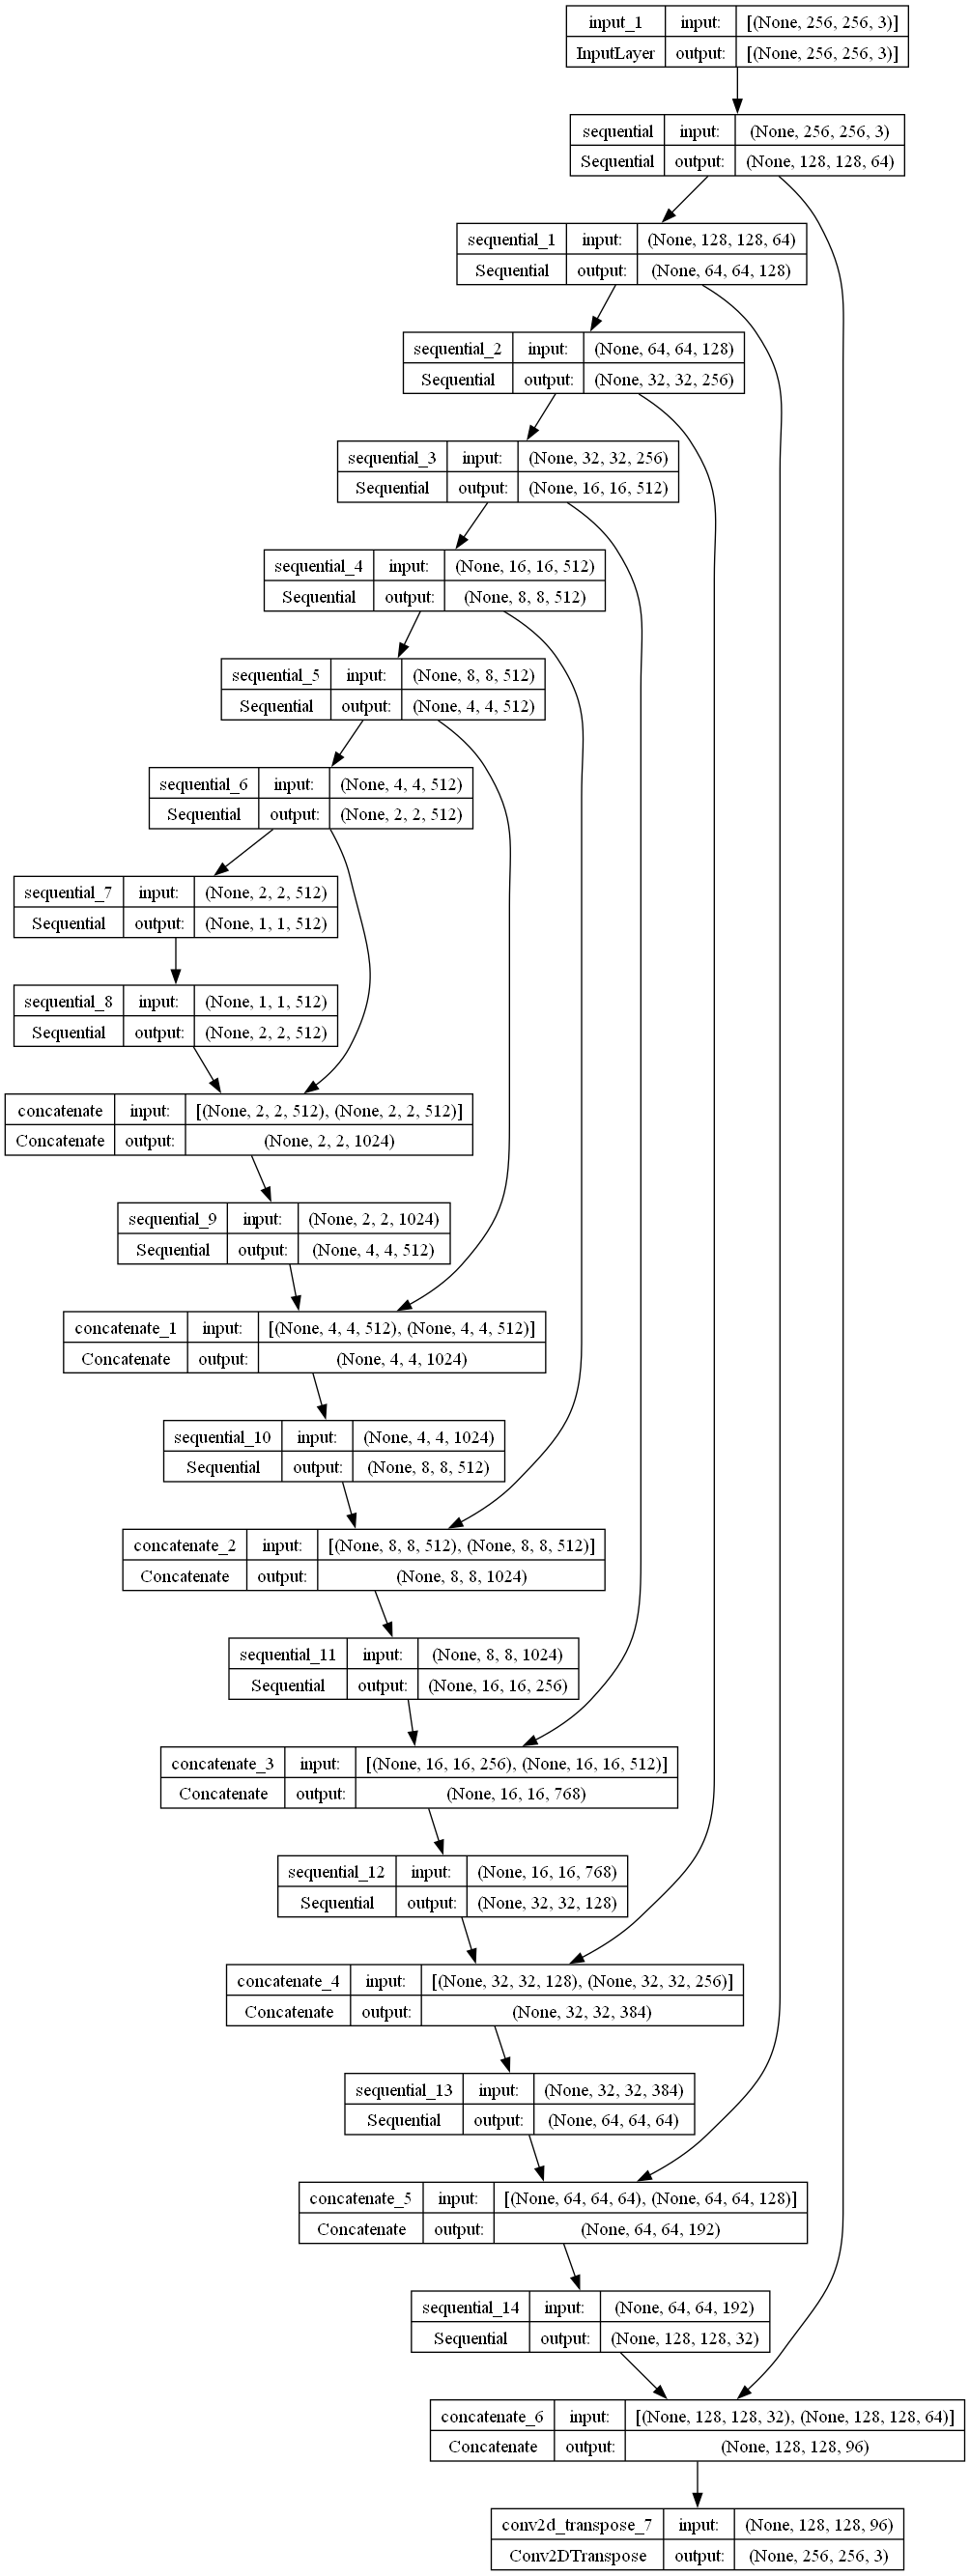
\includegraphics[height=0.95\textheight]{../imgs/cyclegan_generator.png}
        \newpage
    \item \textbf{CycleGAN - Dyskryminator}
        \vspace{3mm} \\
        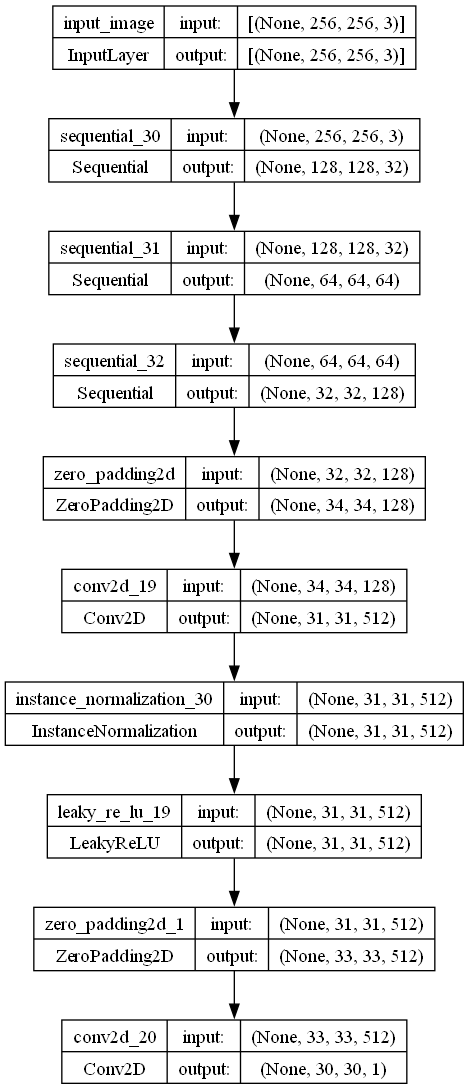
\includegraphics[height=0.95\textheight]{../imgs/cyclegan_discriminator.png}
        \newpage
    \item \textbf{SRGAN - Generator}
        \vspace{3mm} \\
        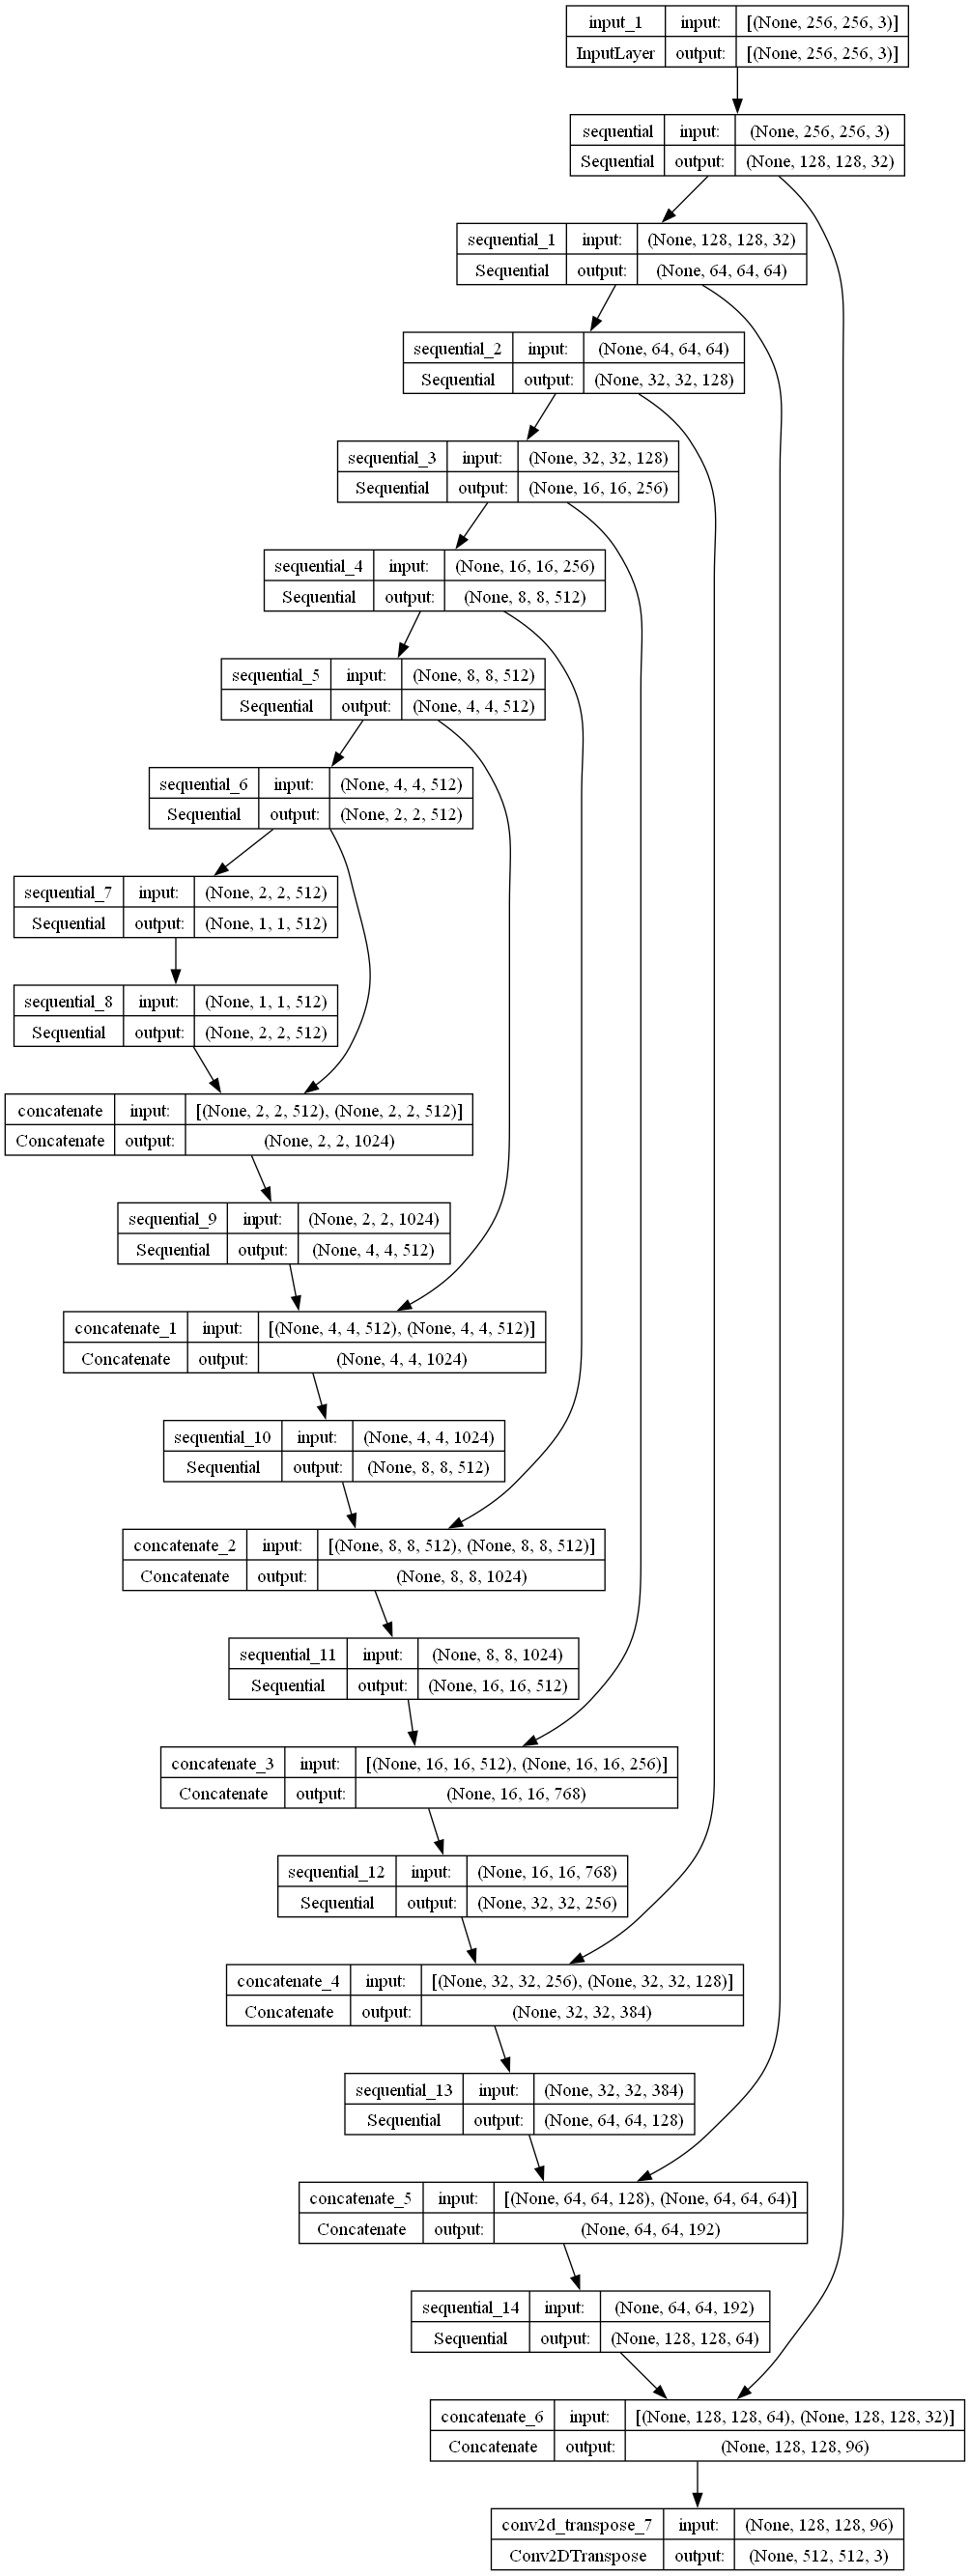
\includegraphics[height=0.95\textheight]{../imgs/srgan_generator.png}
        \newpage
    \item \textbf{SRGAN - Dyskryminator \textit{(PatchGAN)}}
        \vspace{3mm} \\
        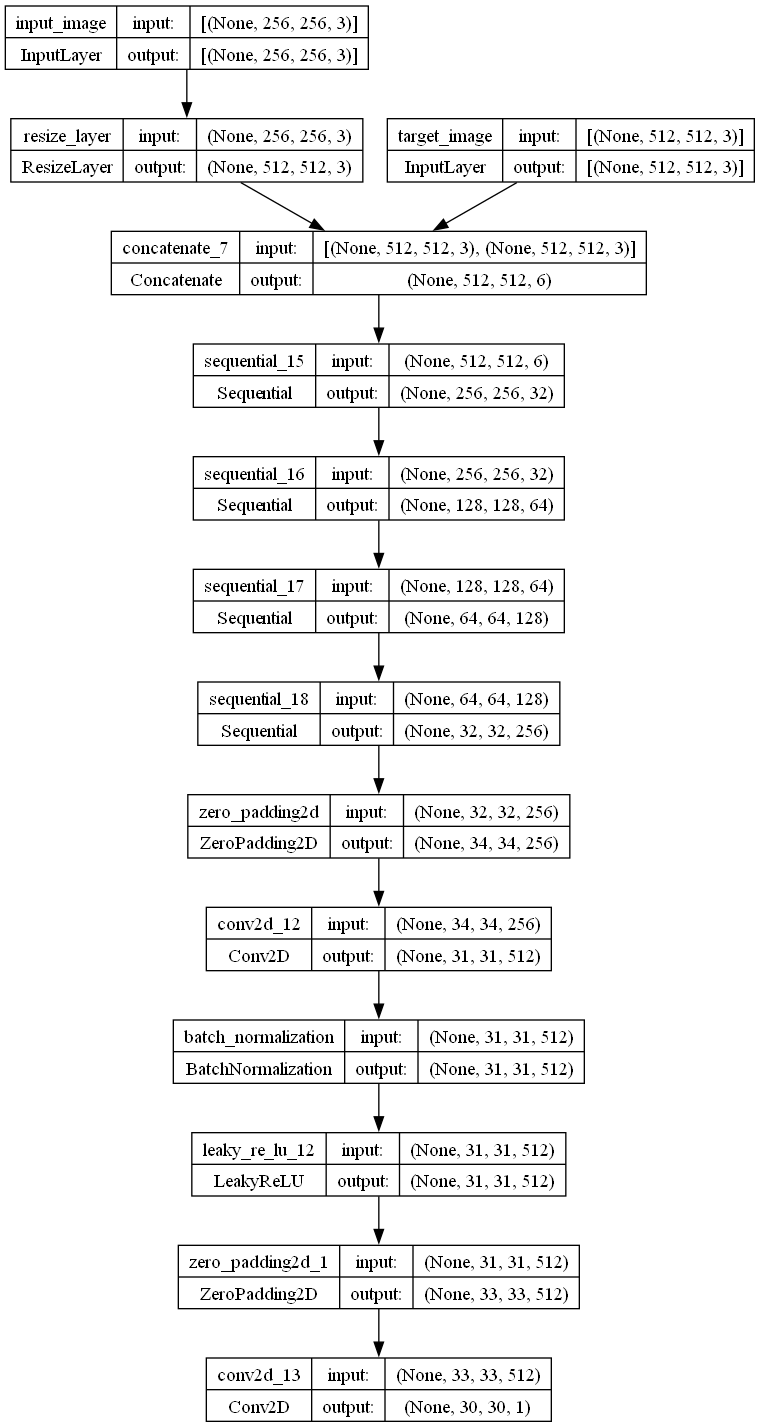
\includegraphics[height=0.95\textheight]{../imgs/srgan_discriminator.png}
        \newpage
\end{enumerate}

\end{document}